\documentclass[../main.tex]{subfiles}

\begin{document}

The selection of certain laser wavelengths can be achived with the introdcution of artificial losses for the undesired remaining wavelengths.

\subsubsection{Birefringent tuner}
    \paragraph{Methodology}
        One possible realisation for these losses is via a birefringent quartz crystal ($n_Q \approx\num{1.55}$ for the main laser line $\lambda = \SI{633}{nm}$). The setup used in the experiment is shown in figure \ref{fig:6-Aufbau}.

        \begin{figure}[H]
            \centering 
            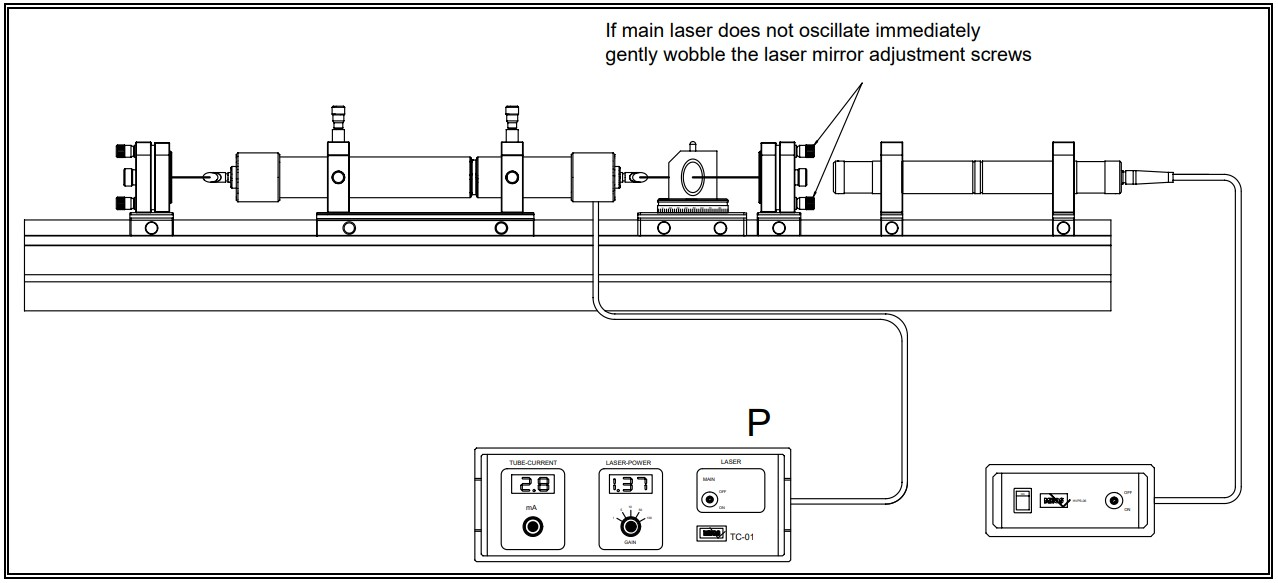
\includegraphics[width = 11cm]{Bilddateien/6-Aufbau.jpg}
            \caption{ Experimental setup for the selection of certain laser wavelengths. The components displayed are from left to right: left laser mirror holder (A), main laser tube (B), birefringent tuner (C), right laser mirror holder (D), pilot laser (E). For the measurment of the laser spectrum a spectrometer can be placed left to the left laser mirror holder (A).}
            \label{fig:6-Aufbau}
        \end{figure}

    \paragraph{Data analysis}

\subsubsection{Fluorescence-spectrum of Neon}
    \paragraph{Methodology}
    \paragraph{Data analysis}

\subsubsection{Littrow prism tuner}
    \paragraph{Methodology}
    \paragraph{Data analysis}

\end{document}